\documentclass[12pt,letter]{article}
\usepackage[moduleName=GBS]{KautenjaDSP}
% import a debugging package to show the margin boxes
% \usepackage{showframe}
% set the graphics path to the img directory
\graphicspath{{img/}}

% algorithm2e stuff
% \SetKwInOut{Objects}{$\CKmatrix{O}$}
% \SetKwInOut{Weights}{$\CKvector{w}$}

\begin{document}
\titlePage{GBS-Logo}{GBS-Module}{KautenjaDSP}

% -------------------
% MARK: Overview
% -------------------

\section{Overview}

GBS is an emulation of the Nintendo GameBoy Sound System (GBS) audio processing unit. The GBS is similar to the Ricoh 2A03, but replaces the triangle waveform generator with a wave-table synthesizer.

GBS provides the key features of the GameBoy Sound System chip, namely,
\begin{itemize}
  \item \textbf{Dual pulse wave generator:} Dual 8-bit pulse waves with four duty cycles: $12.5\%$, $25\%$, $50\%$, and $75\%$
  \item \textbf{Wave-table oscillator:} wave-table synthesis with bit depth of 4 bits and table size of 32 samples. 5 pages of wave-tables can be interpolated between using CV
  \item \textbf{Noise generator:} generate pseudo-random numbers at 7 different frequencies
  \item \textbf{Linear Feedback Shift Register (LFSR):} old-school 8-bit randomness!
\end{itemize}

% -------------------
% MARK: Panel Layout
% -------------------

\clearpage
\section{Panel Layout}

\begin{figure}[!htp]
\centering
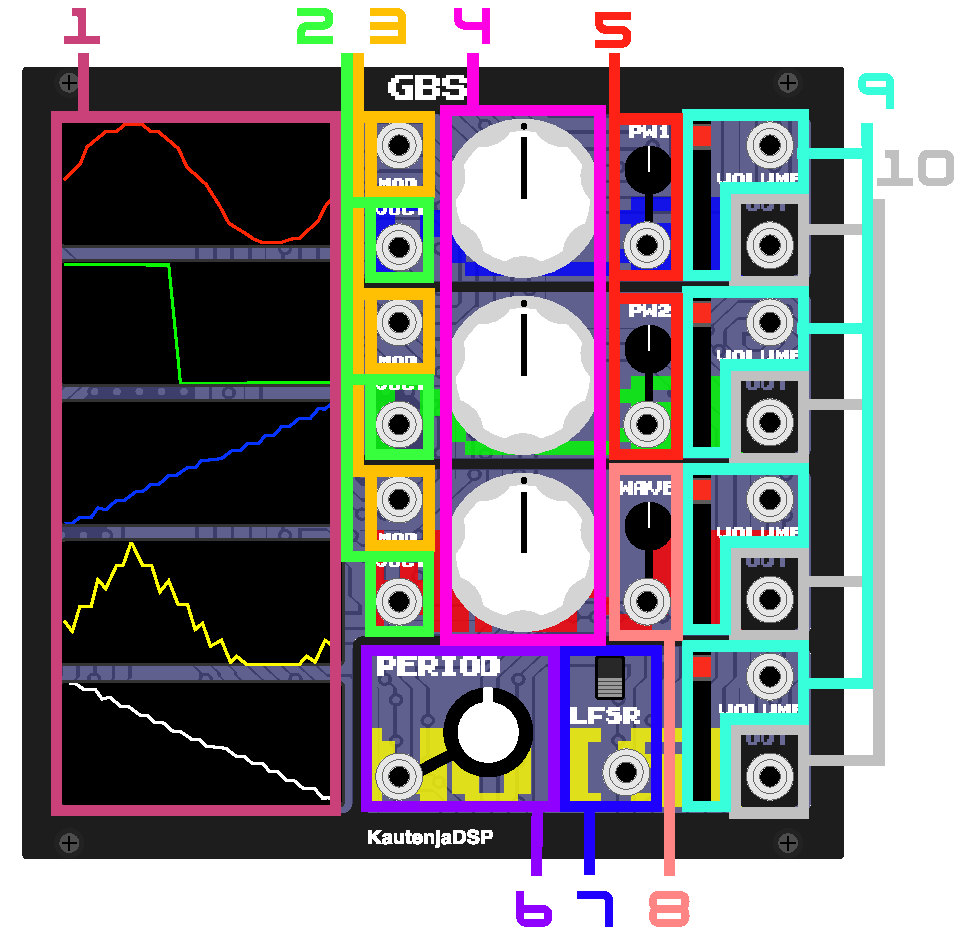
\includegraphics{GBS-Manual}
\end{figure}

\begin{enumerate}
  \item Waveform selection. Draw arbitrary waveforms using the mouse pointer.
  \item $V$/Octave inputs for pulse1, pulse2, and wave-table waveform generators.
  \item linear CV frequency modulation for pulse1, pulse2, and wave-table waveform generators.
  \item Coarse frequency control over the four oscillators.
  \item Pulse width selector. Chooses between four duty cycles: $12.5\%$, $25\%$, $50\%$, and $75\%$ for pulse1 and pulse2.
  \item Period of randomness $\in [0, 7]$ for the noise generator. See \url{https://gbdev.gg8.se/wiki/articles/Gameboy_sound_hardware#Noise_Channel} for approximate frequency and pitch mappings.
  \item CV LFSR gate, high at $2V$. Holds the LFSR generator as long as the input voltage is $>2V$. The switch inverts the direction of the CV input.
  \item Wave-table selection. The big knob determine the wave-table used by the chip. The small knob acts as an attenuverter for the linear CV input. Wave-table morphing is accomplished through 32-bit floating point linear interpolation.
  \item Coarse amplitude control over the oscillators using the 4-bit amplifier.When no input is connected, the slider controls the level from $0\%$ to $100\%$. When an input is connected, the slider acts as an attenuator.
  \item Channel outputs, ${\approx}10V_{pp}$.
\end{enumerate}

% -------------------
% MARK: References
% -------------------

\clearpage
\renewcommand\refname{References \& Acknowledgments}
\nocite{*}
\bibliographystyle{apalike}
\bibliography{references}

\end{document}
